% Borrador para reemplazar la subsección de priorización sucesiva (4.3.7).
% Generado a partir de resultados/ruta_completa/analisis/resumen.json y
% por_parada.csv. No editar los números a mano: regenerar con los scripts.
\subsection{Priorización sucesiva a lo largo de una ruta completa}
\label{ssec:priorizacion_sucesiva}

Para evaluar el lazo completo en un trayecto realista se reprodujo una
misión desde la Av.~La Marina hasta el Instituto Nacional de Salud del Niño,
en Breña: \SI{5.30}{\kilo\meter} de recorrido con trece intersecciones
semaforizadas, cada una con su propia RSU y su propio controlador emulado.
Cada controlador arrancó en un punto aleatorio de su ciclo (\SI{21}{\second}),
de modo que el vehículo encontró condiciones de llegada distintas en cada
intersección. Se ejecutaron tres escenarios en la condición local: A, cinco
repeticiones a velocidad constante de \SI{36}{\kilo\meter\per\hour} con ruido
de posición GNSS; B, cinco repeticiones con un perfil de velocidad
\emph{sintético} variable (20 a \SI{50}{\kilo\meter\per\hour}) y entre tres y
cuatro detenciones, una de ellas forzada a \SI{40}{\meter} de una intersección;
y C, una repetición en la que el vehículo abandona la ruta antes de la octava
intersección.

Las 142 solicitudes emitidas por el servidor fueron concedidas por su RSU,
sin caducidades: la renovación mantuvo cada solicitud vigente con huecos de
como máximo \SI{1.03}{\second} mientras el vehículo avanzaba. En todos los
casos hubo una sola solicitud activa a la vez, salvo cuatro segundos del
escenario C en que dos intersecciones contiguas, separadas
\SI{141}{\meter}, coincidieron tras el reingreso a la ruta. La
Tabla~\ref{tab:ruta_completa} resume los resultados y la
Fig.~\ref{fig:ruta_espacio_tiempo} muestra una repetición del escenario A: el
verde por prioridad se activa en cada intersección antes de la llegada del
vehículo, con independencia de la fase en que se encontraba el plan.

\begin{table}[htbp]
\centering
\caption{Resultados de la priorización sucesiva en la ruta completa (condición local).}
\label{tab:ruta_completa}
\begin{tabular}{lcc}
\hline
 & A (36 km/h) & B (perfil sintético) \\
\hline
Repeticiones / solicitudes & 5 / 65 & 5 / 65 \\
Solicitudes concedidas & 65 & 65 \\
Anticipación real, mediana (s) & 13,0 & 15,0 \\
Anticipación real, mínima (s) & 5,0 & 6,4 \\
Llegadas con anticipación menor a 8 s & 4 de 63 (6,3 \%) & 4 de 64 (6,3 \%) \\
RTT servidor--RSU, mediana (ms) & 37,3 & 31,1 \\
RTT servidor--RSU, 95 \% de los casos bajo (ms) & 63,9 & 70,1 \\
Llegadas en verde sin prioridad (estimado) & 38,1 \% & 40,6 \% \\
Demora evitada por misión (s) & 57,7 & 51,9 \\
\hline
\end{tabular}
\end{table}

\begin{figure}[htbp]
\centering
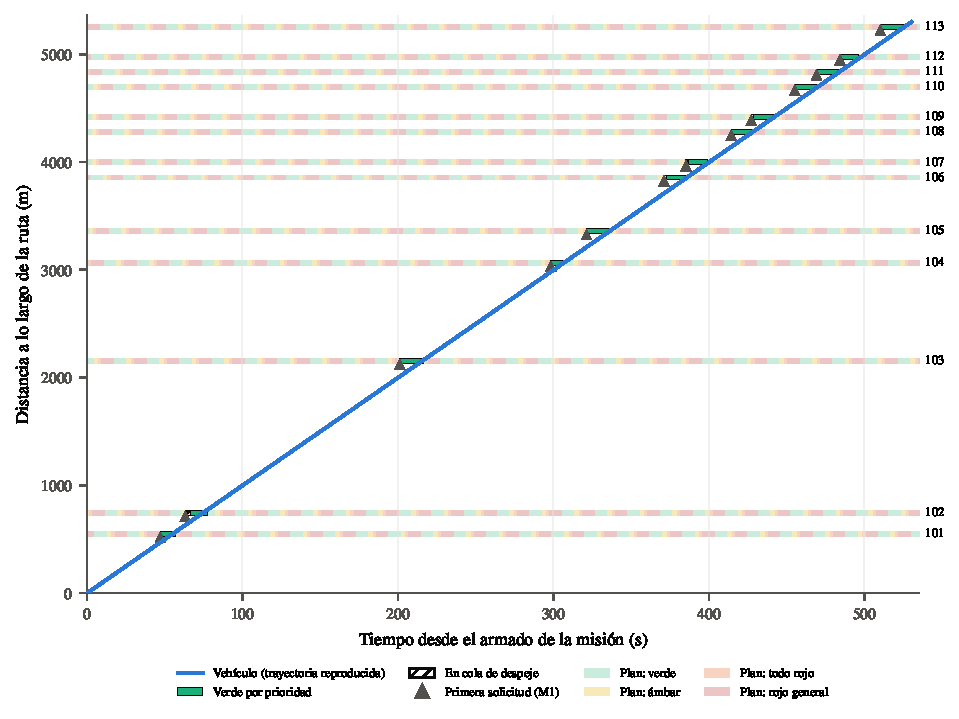
\includegraphics[width=\linewidth]{figuras/fig_ruta_espacio_tiempo_A.pdf}
\caption{Diagrama espacio--tiempo de una repetición del escenario A: plan de
cada controlador (bandas claras), verde por prioridad y primera solicitud a
cada RSU.}
\label{fig:ruta_espacio_tiempo}
\end{figure}

Con prioridad, el vehículo llegó en verde a todas las intersecciones; sin
ella, según la fase que el plan habría tenido en el instante de cruce, solo
lo habría hecho en alrededor del 40~\% de los casos, con una demora evitada
de 52 a \SI{58}{\second} por misión, entre el 8 y el 11~\% del tiempo de
viaje. La mediana de la anticipación real fue de 13 a \SI{15}{\second}, pero
el 6~\% de las llegadas quedó por debajo de los \SI{8}{\second} de
anticipación mínima (Fig.~\ref{fig:ruta_anticipacion}). Hubo dos causas. En
dos intersecciones, la geocerca no confirmó el acceso
antes que el respaldo por ETA, que se evalúa una vez por segundo y emite la
solicitud cuando el ETA ya es menor o igual a \SI{8}{\second}. En el perfil
sintético, a velocidades cercanas a \SI{50}{\kilo\meter\per\hour}, el radio
de \SI{150}{\meter} deja unos \SI{11}{\second}, de los cuales la transición
desde ámbar o todo rojo consume parte antes de que el verde se active.

\begin{figure}[htbp]
\centering
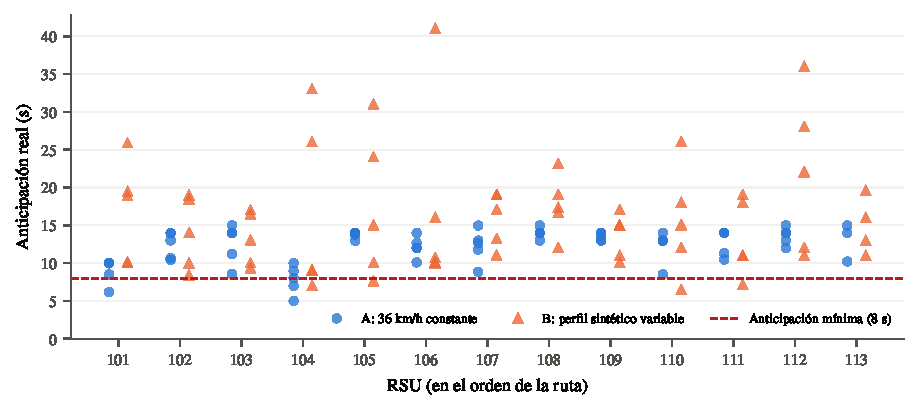
\includegraphics[width=\linewidth]{figuras/fig_ruta_anticipacion.pdf}
\caption{Anticipación real por intersección en los escenarios A y B (perfil
sintético) frente a la anticipación mínima de \SI{8}{\second}.}
\label{fig:ruta_anticipacion}
\end{figure}

En el escenario B el servidor suspendió la solicitud en cuatro de las cinco
detenciones forzadas; en las detenciones ocurridas dentro del radio de la
geocerca, en cambio, la solicitud siguió renovándose y el verde se mantuvo
con el vehículo detenido hasta \SI{20}{\second}. En el escenario C el
servidor recalculó la ruta a los \SI{6}{\second} de la salida, dejó de
solicitar la intersección evitada y retomó la secuencia hasta el destino; la
intersección que el vehículo estaba por abordar al girar recibió un verde de
\SI{1}{\second}, cancelado al detectarse el giro.

Estos resultados tienen límites que deben considerarse: los controladores
son emulados y comparten un mismo ciclo fijo; la trayectoria es reproducida
y no proviene de un vehículo en circulación; el perfil del escenario B es
sintético; y toda la campaña se ejecutó en la condición local, sin el enlace
4G, por lo que los tiempos de red no representan los de campo.
